\section{DNA}
\label{sec:dna}

The essence of life lies in the intricate dance of \acs{DNA}, or deoxyribonucleic acid, a molecule located in the nucleus of every cell. This molecule is, in fact, a macro-molecule and is easily identified by its characteristic double-helix shape consisting of two nucleotide chains. Each nucleotide that makes up the chain consists of a sugar-phosphate molecule and a nitrogenous base. We recognise four nitrogenous bases, Adenine, Cytosine, Guanine and Thymine, which bind two by two through hydrogen bonds forming specific pairs, as illustrated in Figure~\ref{fig:DNA-double-helix-structure}: Adenine and Thymine (A-T), Cytosine and Guanine (C-G). The order in which the nitrogenous bases follow one another along the nucleotide chain orchestrates the symphony of existence.

\begin{figure}[!ht]
	\centering
	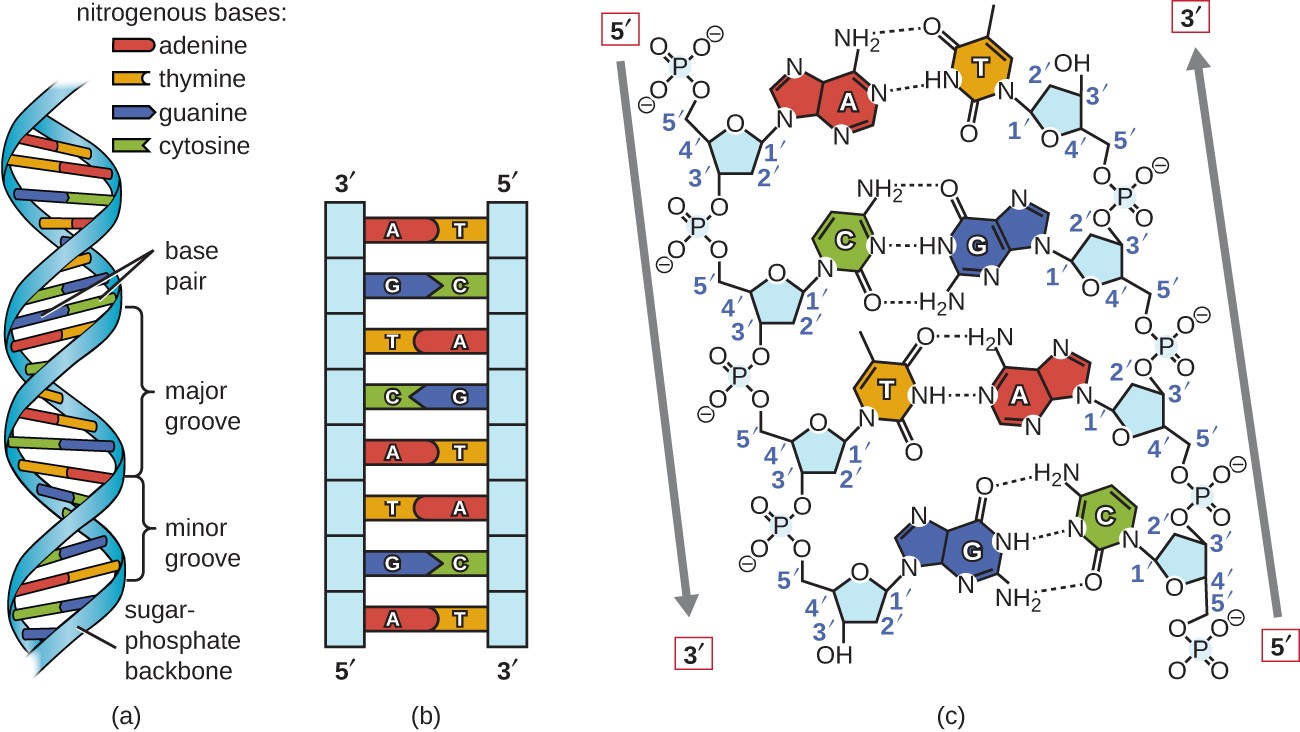
\includegraphics[width=0.85\linewidth]{images/dna-structure}
	\caption[The fundamental structure of the \acs{DNA}]{The fundamental structure of the \acs{DNA} double helix consists of two strands, each composed of chains of nucleotides. Within this framework, every nucleotide forms a bond with its complementary counterpart on the opposing strand \cite{openstax2016microbiology}.}
	\label{fig:DNA-double-helix-structure}
\end{figure}




\subsection{DNA sequencing}
\label{subsec:dna-sequencing}

\acs{DNA} sequencing is the process of determining the nucleotide sequence of a \acs{DNA} fragment, and is fundamental to genetic research, molecular biology, medicine and other disciplines. Numerous technologies have been developed over the years to make this process faster, more accurate and more accessible. Costs have also fallen dramatically (Figure~\ref{fig:sequencing-cost-per-human-genome} and Figure~\ref{fig:sequencing-cost-per-mb}): from the Human Genome Project, which required billions of dollars, we have moved on to technologies that allow the sequencing of an entire human genome for less than \$1,000. The cost, of course, varies depending on the technology used, the coverage required and the complexity of the project \cite{nhgri2023cost}. \acs{NGS} platforms such as Illumina and Ion Torrent offer inexpensive options for large-scale projects, while technologies such as \acs{PacBio}, while more expensive, provide unique details for specific needs. The main sequencing techniques are described below.

\begin{figure}[!ht]
	\centering
	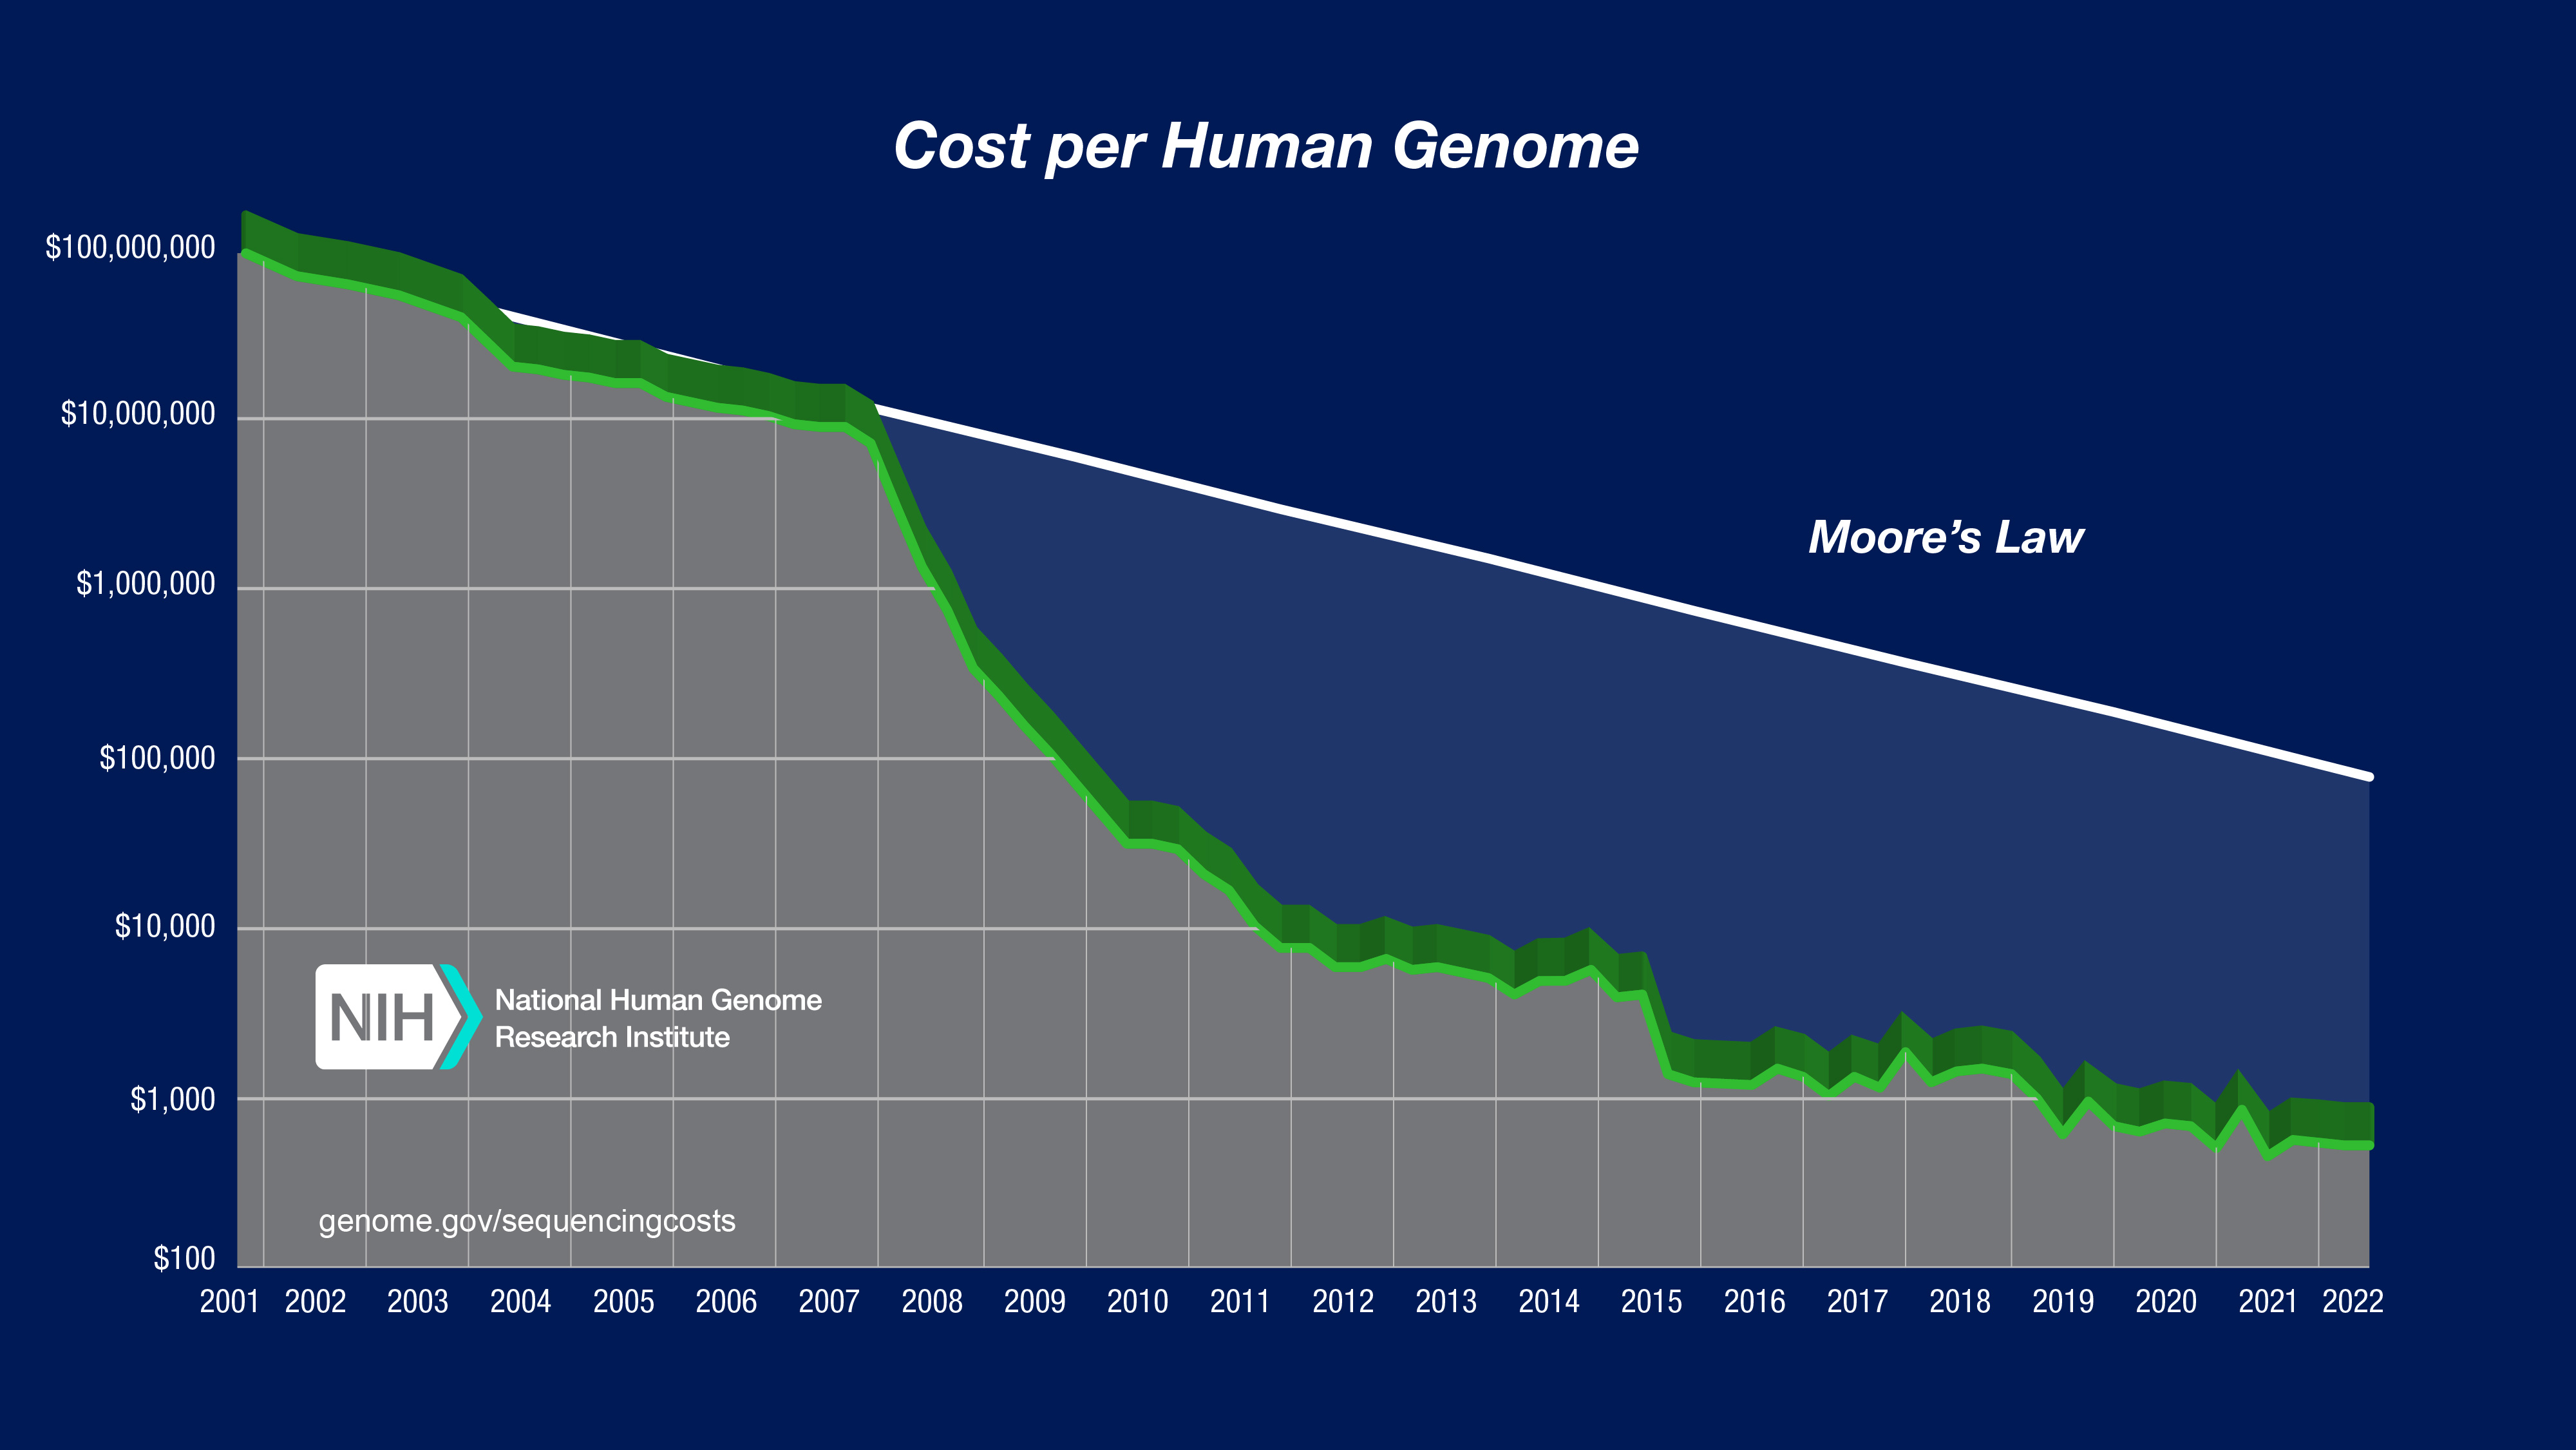
\includegraphics[width=0.85\linewidth]{images/2022_Sequencing_cost_per_Human_Genome}
	\caption[Sequencing cost per genome data]{Sequencing cost per genome data - 2022: the cost per genome has become much lower than Moore’s Law \cite{nhgri2023cost}.}
	\label{fig:sequencing-cost-per-human-genome}
\end{figure}

\begin{figure}[!ht]
	\centering
	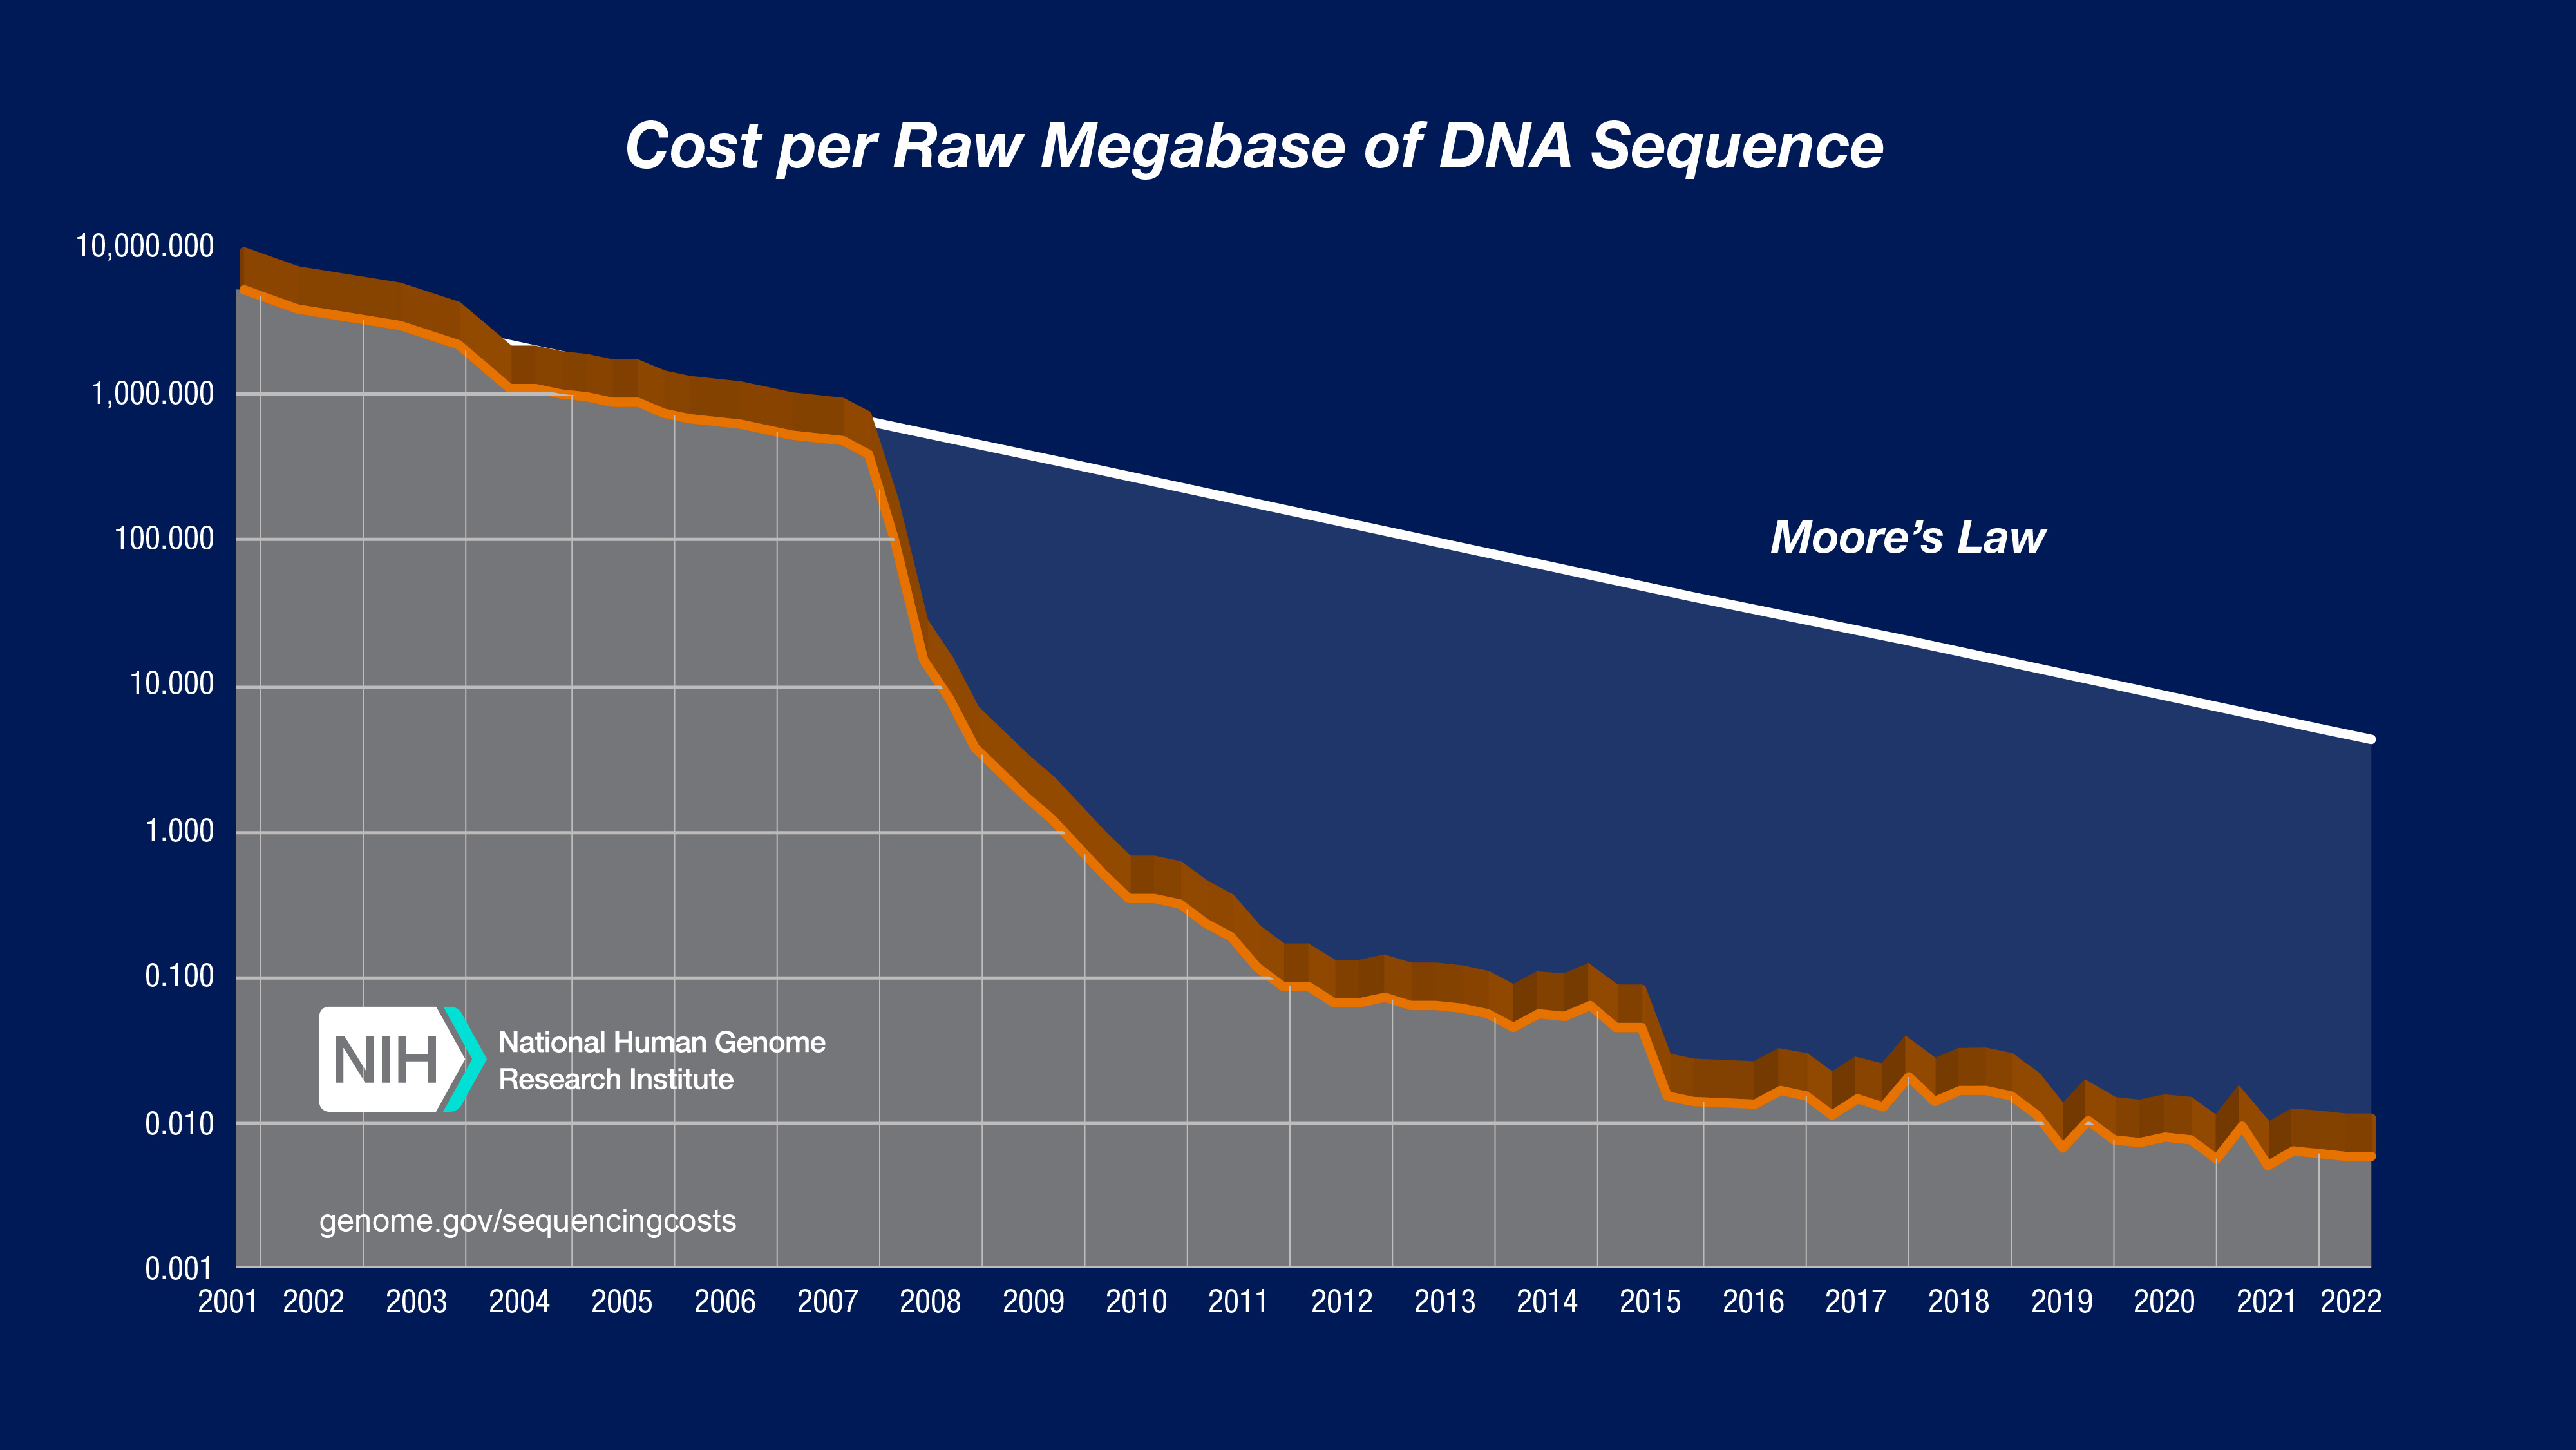
\includegraphics[width=0.85\linewidth]{images/2022_Sequencing_cost_per_Mb}
	\caption[Sequencing cost per megabase]{Sequencing cost per megabase - 2022: the cost per megabase has become much lower than Moore’s Law \cite{nhgri2023cost}.}
	\label{fig:sequencing-cost-per-mb}
\end{figure}


	\subsubsection{Sanger Method}
	The Sanger method \cite{sanger1977dna}, developed by Frederick Sanger in the 1970s, was the first successful approach to \acs{DNA} sequencing. It utilises chain termination, where \ac{ddNTPs} interrupt \acs{DNA} synthesis, allowing the sequence to be read according to the length of the fragments obtained. Although accurate, the Sanger method is relatively slow and expensive, suitable mainly for shorter \acs{DNA} sequences. This method was used for the Human Genome Project, which sequenced the entire human genome at a cost of approximately \$2.7 billion.
	
	
	\subsubsection{Next-Generation Sequencing}
	In recent decades, \ac{NGS} technologies \cite{shendure2008nextgeneration,satam2023nextgeneration} have revolutionised the field, enabling massive, parallel sequencing of billions of \acs{DNA} fragments. Among the \acs{NGS} platforms, Illumina, Ion Torrent and \acs{PacBio} stand out.
	
	\begin{figure}[!ht]
		\centering
		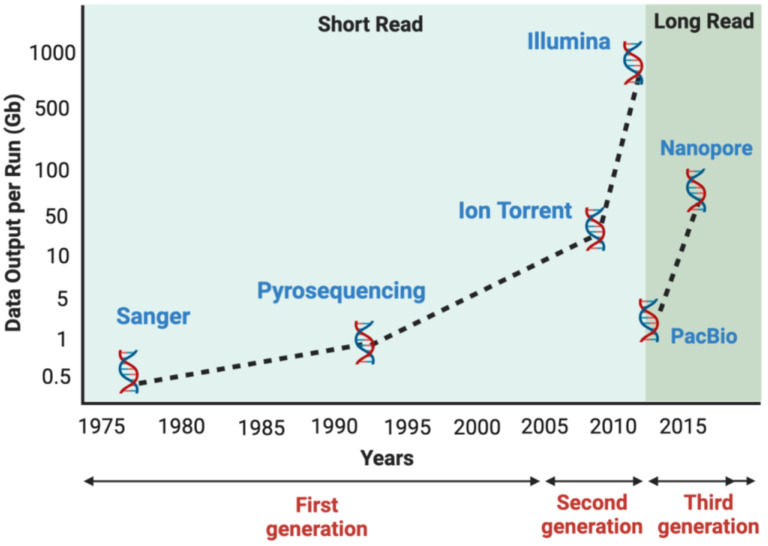
\includegraphics[width=0.85\linewidth]{images/next-generation_sequencing_technology}
		\caption[Evolution of sequencing technologies]{Evolution of sequencing technologies \cite{satam2023nextgeneration}.}
		\label{fig:evolution-sequencing-technologies}
	\end{figure}

	\textbf{Illumina} is one of the leaders in the \acs{NGS} market. It uses \ac{SBS} technology, where fluorescently labelled nucleotides are incorporated into \acs{DNA}, and fluorescent images reveal the sequence. This method offers high accuracy and read depth, making it ideal for large-scale genomics projects. The cost to sequence a complete human genome with Illumina can range from a few hundred to a few thousand dollars, depending on the coverage and specifications of the project.
	
	The \textbf{Ion Torrent} technology, developed by Life Technologies, is based on the detection of hydrogen ion release during nucleotide incorporation. This fluorescence-free approach allows rapid and low-cost sequencing. Although accuracy may be lower than Illumina, Ion Torrent is advantageous for applications requiring speed and low cost.
	
	\textbf{Pacific Biosciences} (\acs{PacBio}) has introduced \ac{SMRT} Sequencing technology. It offers the ability to read long \acs{DNA} sequences, with reads that can exceed 10,000 bases. This is particularly useful for the assembly of genomes, but also for the analysis of complex repetitive regions. Despite its higher costs compared to other \acs{NGS} technologies, \acs{PacBio} is useful for studies requiring long and detailed reads.



	\subsection{Assembly Techniques}
	\label{subsec:assembly-techniques}
	
	\acs{DNA} sequencing produces fragments, called \emph{reads}, that must be assembled to reconstruct the original sequence. These are the two main assembly strategies:
	\begin{itemize}
		\item \textbf{de novo assembly} \cite{nagarajan2013sequence} is used when no reference sequence is available. Fragments are assembled based only on the overlaps between them. This technique is essential for sequencing new genomes.
		
		\item In \textbf{reference assembly}, mainly used for genetic variability studies, fragments are aligned to an existing reference sequence. This facilitates the assembly process and improves accuracy.
	\end{itemize}
